\documentclass[12pt,letterpaper]{article}
\usepackage[utf8]{inputenc}
\usepackage[spanish]{babel}
\usepackage{amsmath}
\usepackage{amsfonts}
\usepackage{amssymb}
\usepackage{graphicx}
\usepackage{geometry}
\usepackage{hyperref}
\usepackage{listings}
\usepackage{xcolor}
\usepackage{booktabs}
\usepackage{float}

\geometry{margin=1in}

\definecolor{codegray}{rgb}{0.5,0.5,0.5}
\definecolor{codeprimary}{rgb}{0.1,0.2,0.6}
\definecolor{backcolour}{rgb}{0.95,0.95,0.92}

\lstdefinestyle{mystyle}{
    backgroundcolor=\color{backcolour},   
    commentstyle=\color{codegray}\itshape,
    keywordstyle=\color{codeprimary}\bfseries,
    numberstyle=\tiny\color{codegray},
    stringstyle=\color{orange},
    basicstyle=\ttfamily\footnotesize,
    breakatwhitespace=false,         
    breaklines=true,                 
    captionpos=b,                    
    keepspaces=true,                 
    numbers=left,                    
    numbersep=5pt,                  
    showspaces=false,                
    showstringspaces=false,
    showtabs=false,                  
    tabsize=2
}
\lstset{style=mystyle}

\title{
    \textbf{Informe Técnico: Simulador RV32I en Python}\\
    \large{Simulación de Arquitectura de Computadores Basada en Módulos de Hardware (Verilog a Python)}
}
\author{Antonio}
\date{\today}

\begin{document}

\maketitle

\begin{abstract}
Este informe describe el diseño y desarrollo de un simulador educativo para el conjunto de instrucciones (ISA) RISC-V de 32 bits (RV32I). La estrategia de diseño se centró en la traducción funcional directa de los bloques constructivos de hardware descritos originalmente en Verilog hacia funciones estructuradas de Python. Este enfoque modular permite emular el comportamiento combinacional y secuencial ciclo a ciclo de una CPU monociclo (Single-Cycle). Se integró además una interfaz de desarrollo web (IDE) utilizando Next.js y componentes de shadcn/ui que proporciona depuración paso a paso (step-forward y step-back), visualización dinámica de registros, editor de memoria hexadecimal y desensamblado dinámico mediante Capstone. El backend utiliza FastAPI y ofrece autenticación con Google Login para control de accesos. El simulador fue validado con tres programas complejos de prueba, confirmando un comportamiento exacto al del hardware.
\end{abstract}

\newpage
\tableofcontents
\newpage

\section{Introducción}
El estudio práctico de la arquitectura de computadores requiere herramientas de simulación que ayuden a los estudiantes a comprender la interacción entre el camino de datos (datapath), la unidad de control y la memoria. Si bien las herramientas basadas en lenguajes de descripción de hardware (HDL) como Verilog o VHDL son el estándar de la industria, su curva de aprendizaje y la dificultad para integrarse con interfaces gráficas web dinámicas limitan su uso en laboratorios interactivos de software.

Este proyecto implementa un simulador monociclo del procesador RISC-V (RV32I) utilizando una estrategia novedosa: traducir de manera funcional todos los módulos de hardware escritos en Verilog directamente a módulos y scripts equivalentes en Python. El resultado es un simulador que emula el ciclo de reloj de hardware pero corre nativamente en un backend web liviano, acoplándose de manera interactiva a un frontend moderno.

---

\section{Estrategia de Diseño: De Verilog a Python}
Para mantener la fidelidad física y conceptual del procesador, no se utilizó un emulador abstracto a nivel de software. En su lugar, se tradujeron uno a uno los bloques lógicos de Verilog del procesador monociclo. 

\subsection{Mapeo de Módulos de Hardware}
Cada archivo de hardware en Verilog se convirtió en una función puramente matemática/lógica en Python, conservando las señales de entrada y salida:

\begin{itemize}
    \item \textbf{flopr (Registro de Estado):} Traducido a una función secuencial con señales de control de reset y carga. Representa el registro que mantiene el valor del PC.
    \item \textbf{mux2 (Multiplexor):} Simula la selección física entre dos buses de datos basada en una línea de control.
    \item \textbf{extend (Unidad de Extensión de Signo):} Decodifica los inmediatos empaquetados del formato RISC-V (I, S, B, U, J) y les aplica extensión de signo de 32 bits.
    \item \textbf{alu (Unidad Aritmético-Lógica):} Modela la ALU con sumadores, restadores, compuertas AND/OR/XOR y desplazadores lógicos/aritméticos (SLL, SRL, SRA).
    \item \textbf{control\_unit (Unidad de Control):} Decodifica los campos \texttt{opcode}, \texttt{funct3} y \texttt{funct7} de la instrucción y genera todas las señales de control de hardware (\texttt{RegWrite}, \texttt{ALUSrc}, \texttt{MemWrite}, \texttt{ResultSrc}, \texttt{Jump}, \texttt{BranchType}).
    \item \textbf{datapath (Camino de Datos):} El bloque combinacional principal que interconecta la ALU, los multiplexores, el banco de registros y el sumador de saltos del PC.
\end{itemize}

\subsection{El Ciclo de Reloj Simulado}
El bucle principal del simulador emula el flanco de subida del reloj (\textit{rising edge}) en una función secuencial que repite cuatro fases secuenciales:

\begin{lstlisting}[language=Python, caption=Bucle secuencial del ciclo de reloj simulado en Python]
# 1. FETCH (Leer Instruccion de la Memoria ROM)
Instr = INSTRUCTION_MEMORY(PC)

# 2. DECODE (Unidad de Control genera senales combinacionales)
ImmSrc, RegWrite, ALUSrc, ALUControl, MemWrite, ResultSrc, Jump, BranchType = CONTROL_UNIT(Instr)

# 3. EXECUTE (El Datapath interconecta registros, ALU y calcula direcciones)
PCNext, ALUResult, WriteData, Zero, ImmExt, a3, PCPlus4, PCTarget, PCSrc = DATAPATH(
    PC, Instr, ImmSrc, ALUSrc, ALUControl, ResultSrc, Jump, BranchType
)

# 4. MEMORY / WRITEBACK (Lectura/Escritura en RAM y escritura en Banco de Registros)
ReadData = DATA_MEMORY(ALUResult, WriteData, MemWrite, funct3)
Result = MUX2(ALUResult, ReadData, ResultSrc)
WRITE_REGISTER_FILE(a3, Result, RegWrite)

# Actualizacion del PC en el flanco del reloj
PC = FLOPR(PCNext, reset, width=32)
\end{lstlisting}

---

\section{Estructura de Memoria y CPU}
El simulador cuenta con dos memorias separadas:
\begin{enumerate}
    \item \textbf{Memoria de Instrucciones:} Indexada en palabras de 32 bits, almacena el programa compilado. Se redimensiona de forma dinámica según el largo del programa.
    \item \textbf{Memoria de Datos:} Representada por un bloque plano de \textbf{8 KB (8192 bytes)}. El direccionamiento es por byte (byte-addressable) permitiendo alineamientos exactos.
\end{enumerate}

\subsection{Endianness y Operaciones de Memoria}
El simulador respeta la convención \textbf{Little-Endian} del estándar de RISC-V. La lectura y escritura física se maneja a nivel de bytes individuales:
\begin{itemize}
    \item Cargas firmadas y no firmadas: \texttt{lb}, \texttt{lh}, \texttt{lw}, \texttt{lbu}, \texttt{lhu}.
    \item Guardados de datos: \texttt{sb}, \texttt{sh}, \texttt{sw}.
\end{itemize}

---

\section{Instrucciones RV32I Soportadas}
El conjunto de instrucciones emulado comprende la base de enteros del RISC-V (RV32I):

\begin{table}[H]
\centering
\caption{Instrucciones del ISA soportadas por el simulador}
\begin{tabular}{lll}
\toprule
\textbf{Categoría} & \textbf{Instrucciones} & \textbf{Descripción} \\
\midrule
Tipo R & \texttt{add, sub, sll, slt, sltu, xor, srl, sra, or, and} & Operaciones Aritmético-Lógicas \\
Tipo I ALU & \texttt{addi, slti, sltiu, xori, ori, andi, slli, srli, srai} & Aritmética con Inmediatos \\
Cargas (Loads) & \texttt{lb, lh, lw, lbu, lhu} & Lecturas Little-Endian firmadas/sin signo \\
Escrituras (Stores) & \texttt{sb, sh, sw} & Escritura de bytes, media palabra y palabras \\
Branches (Tipo B) & \texttt{beq, bne, blt, bge, bltu, bgeu} & Saltos condicionales firmados/sin signo \\
Tipo U & \texttt{lui, auipc} & Carga de inmediatos de 20 bits en parte alta \\
Tipo J y I Jumps & \texttt{jal, jalr} & Saltos incondicionales y llamadas a funciones \\
Sistema & \texttt{ecall} & Llamada al sistema (Consola virtual) \\
\bottomrule
\end{tabular}
\end{table}

---

\section{Arquitectura Tecnológica del Proyecto}

El simulador se divide en una arquitectura desacoplada Cliente-Servidor (Frontend-Backend) moderna, interactiva y escalable.

\subsection{Tecnologías del Frontend}
El frontend está diseñado como una aplicación web de página única (SPA) estructurada de la siguiente manera:
\begin{itemize}
    \item \textbf{Next.js 16.2 (React 19) y TypeScript:} Proporciona la estructura del IDE, el enrutamiento seguro de vistas y un tipado estático que evita errores en tiempo de ejecución.
    \item \textbf{shadcn/ui y Tailwind CSS:} Se emplearon componentes interactivos basados en Radix Primitives estilizados con Tailwind (como diálogos modal, tablas, acordeones, y botones) para dar una estética retro-futurista, consistente y profesional al IDE.
    \item \textbf{Google Login (OAuth 2.0):} Integración del flujo de autenticación federada de Google en el frontend para permitir accesos autenticados a las herramientas del simulador.
\end{itemize}

\subsection{Tecnologías del Backend}
El backend actúa como el motor de ejecución del hardware virtual y la API de control:
\begin{itemize}
    \item \textbf{FastAPI (Python):} Framework de alto rendimiento utilizado para exponer servicios REST. Gestiona las sesiones interactivas de depuración almacenando el estado de la simulación en memoria.
    \item \textbf{Capstone Engine:} Usado para decodificar e inspeccionar en lenguaje natural los bytes que ejecuta la CPU virtual.
    \item \textbf{Base de Datos y Autenticación:} Soporte para persistencia en base de datos SQLAlchemy/PostgreSQL, encargado de validar las credenciales de sesión del Google OAuth y gestionar el perfil de usuario.
\end{itemize}

---

\section{Resultados de Validación y Evidencias}
A continuación se presentan las evidencias directas del funcionamiento del simulador capturadas desde la interfaz web final.

\subsection{Entorno de Trabajo e IDE General}
La interfaz del IDE proporciona una vista integrada del código fuente, la terminal virtual y los paneles de inspección del hardware.

\begin{figure}[H]
    \centering
    
\includegraphics[width=0.95\textwidth]{images/image.png}
    \caption{Vista general del IDE con código cargado y panel de registros en formato decimal.}
    \label{fig:ide_general}
\end{figure}

El IDE permite configurar límites de pasos de simulación, formato de visualización (hexadecimal o decimal) y filtros para la visualización de registros con valor cero.

\begin{figure}[H]
    \centering
    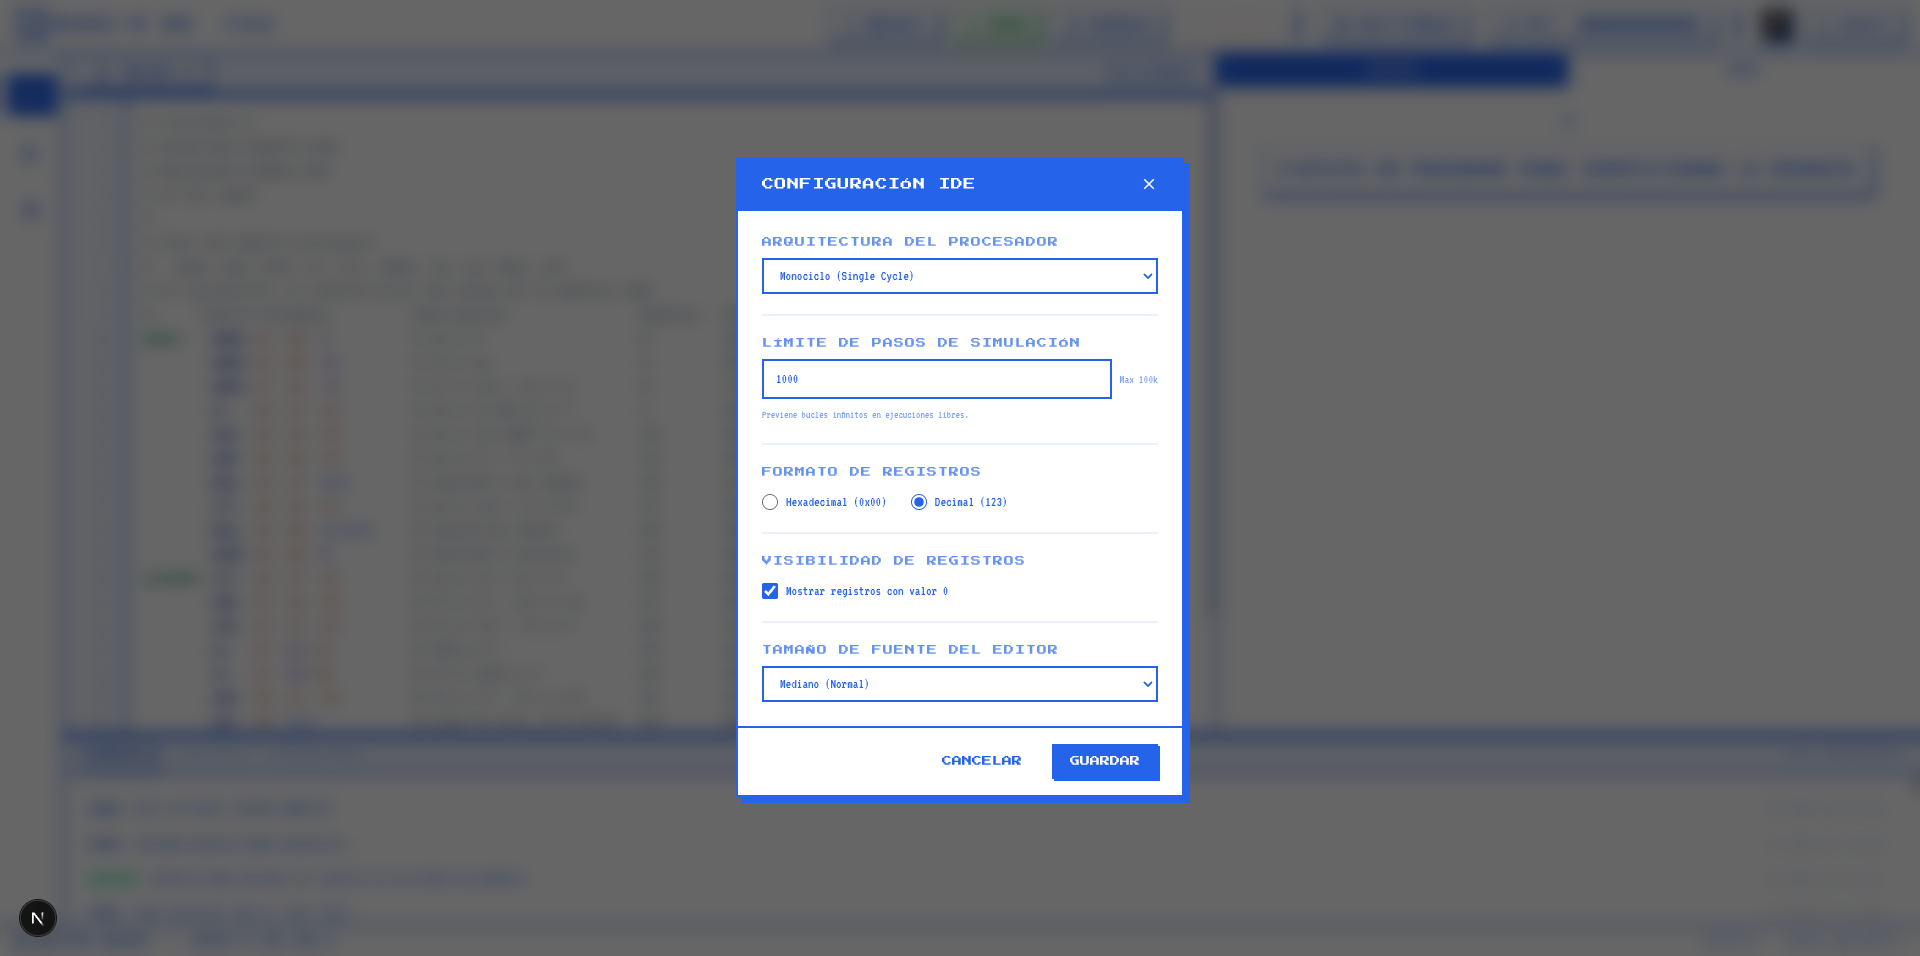
\includegraphics[width=0.75\textwidth]{images/configuration_ide.png}
    \caption{Modal de configuraciones del IDE (Settings).}
    \label{fig:config_ide}
\end{figure}

\subsection{Inspección de Registros y Depuración}
Durante las pruebas se puede visualizar dinámicamente cómo varían los valores de los registros en base hexadecimal o decimal.

\begin{figure}[H]
    \centering
    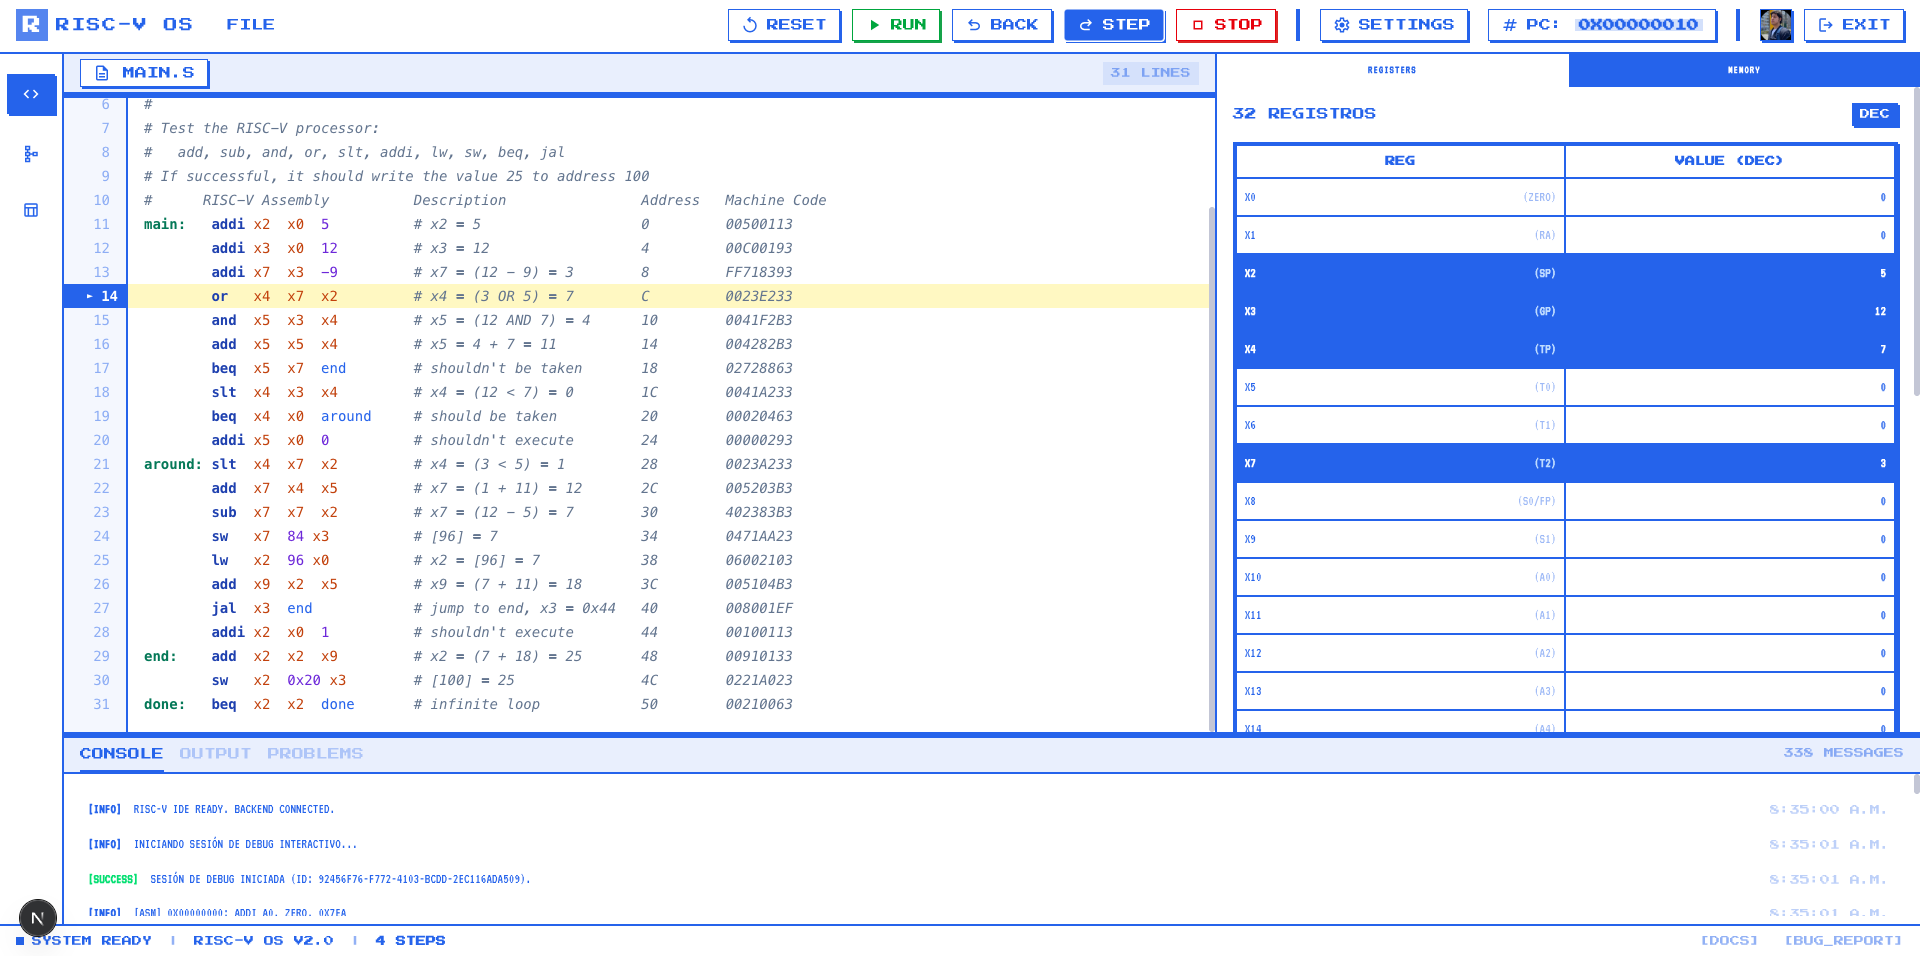
\includegraphics[width=0.85\textwidth]{images/debug_register.png}
    \caption{Panel de visualización de los 32 registros físicos del procesador en modo debug.}
    \label{fig:debug_register}
\end{figure}

\subsection{Inspección de Memoria RAM}
El mapa de memoria permite examinar el contenido hexadecimal de la RAM en bloques de 16 bytes, indicando las etiquetas del PC y el SP correspondientes.

\begin{figure}[H]
    \centering
    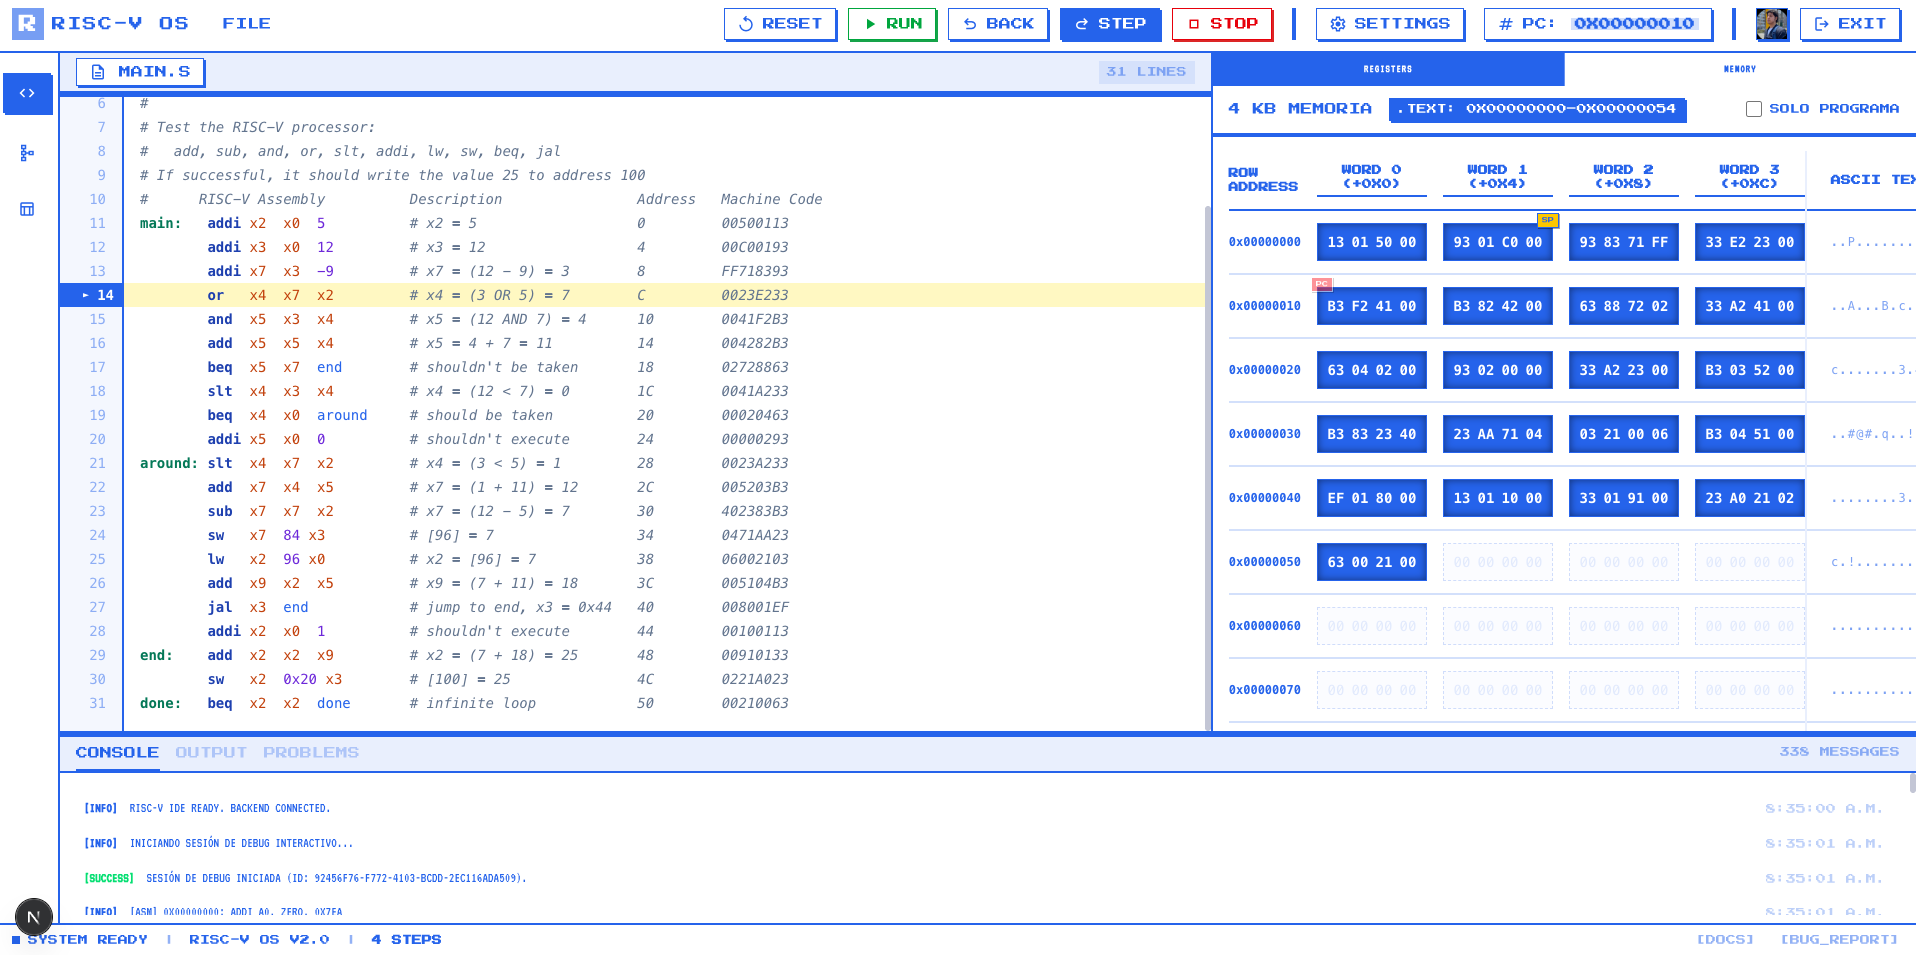
\includegraphics[width=0.95\textwidth]{images/debug_memory.png}
    \caption{Mapa hexadecimal de memoria con indicadores visuales interactivos de PC y SP.}
    \label{fig:debug_memory}
\end{figure}

\subsection{Ejecución de Algoritmos Complejos}
Se validó la simulación con algoritmos recursivos que hacen uso intensivo de la pila de memoria y el banco de registros.

\begin{figure}[H]
    \centering
    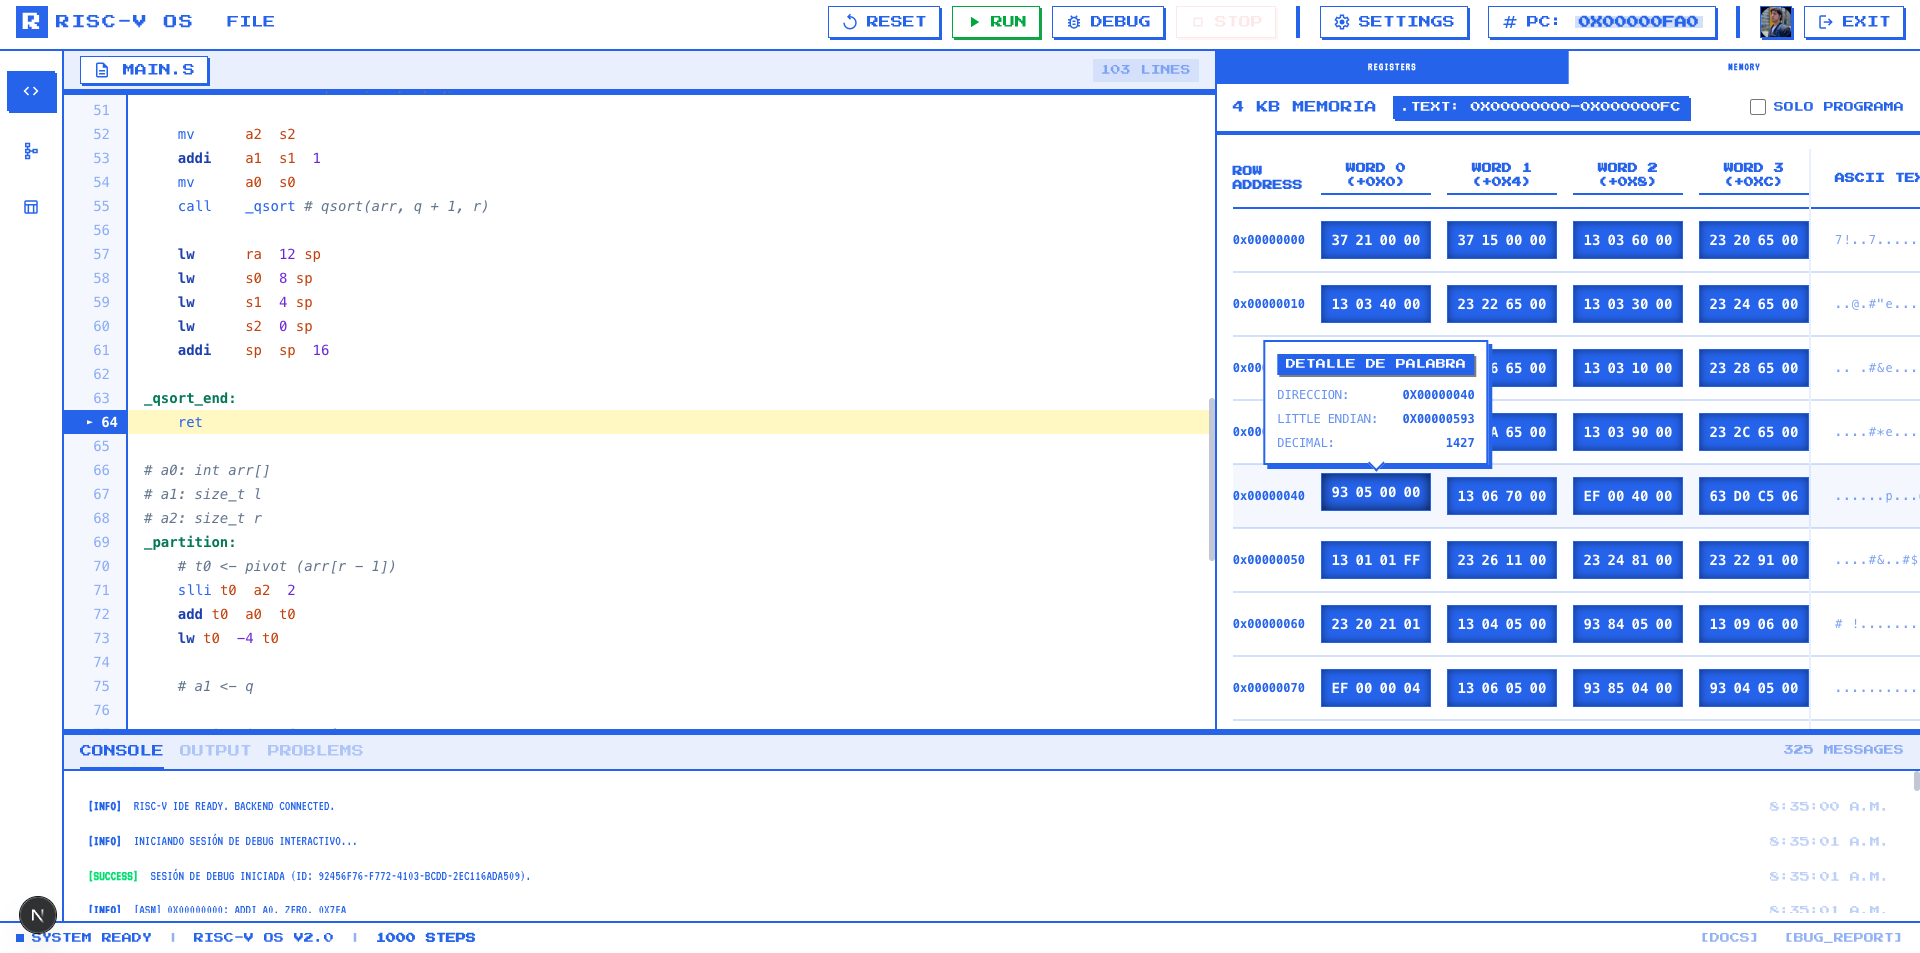
\includegraphics[width=0.95\textwidth]{images/quicksort.png}
    \caption{Validación exitosa del algoritmo Quicksort en el simulador, ordenando la memoria en 0x1000.}
    \label{fig:quicksort}
\end{figure}

\begin{figure}[H]
    \centering
    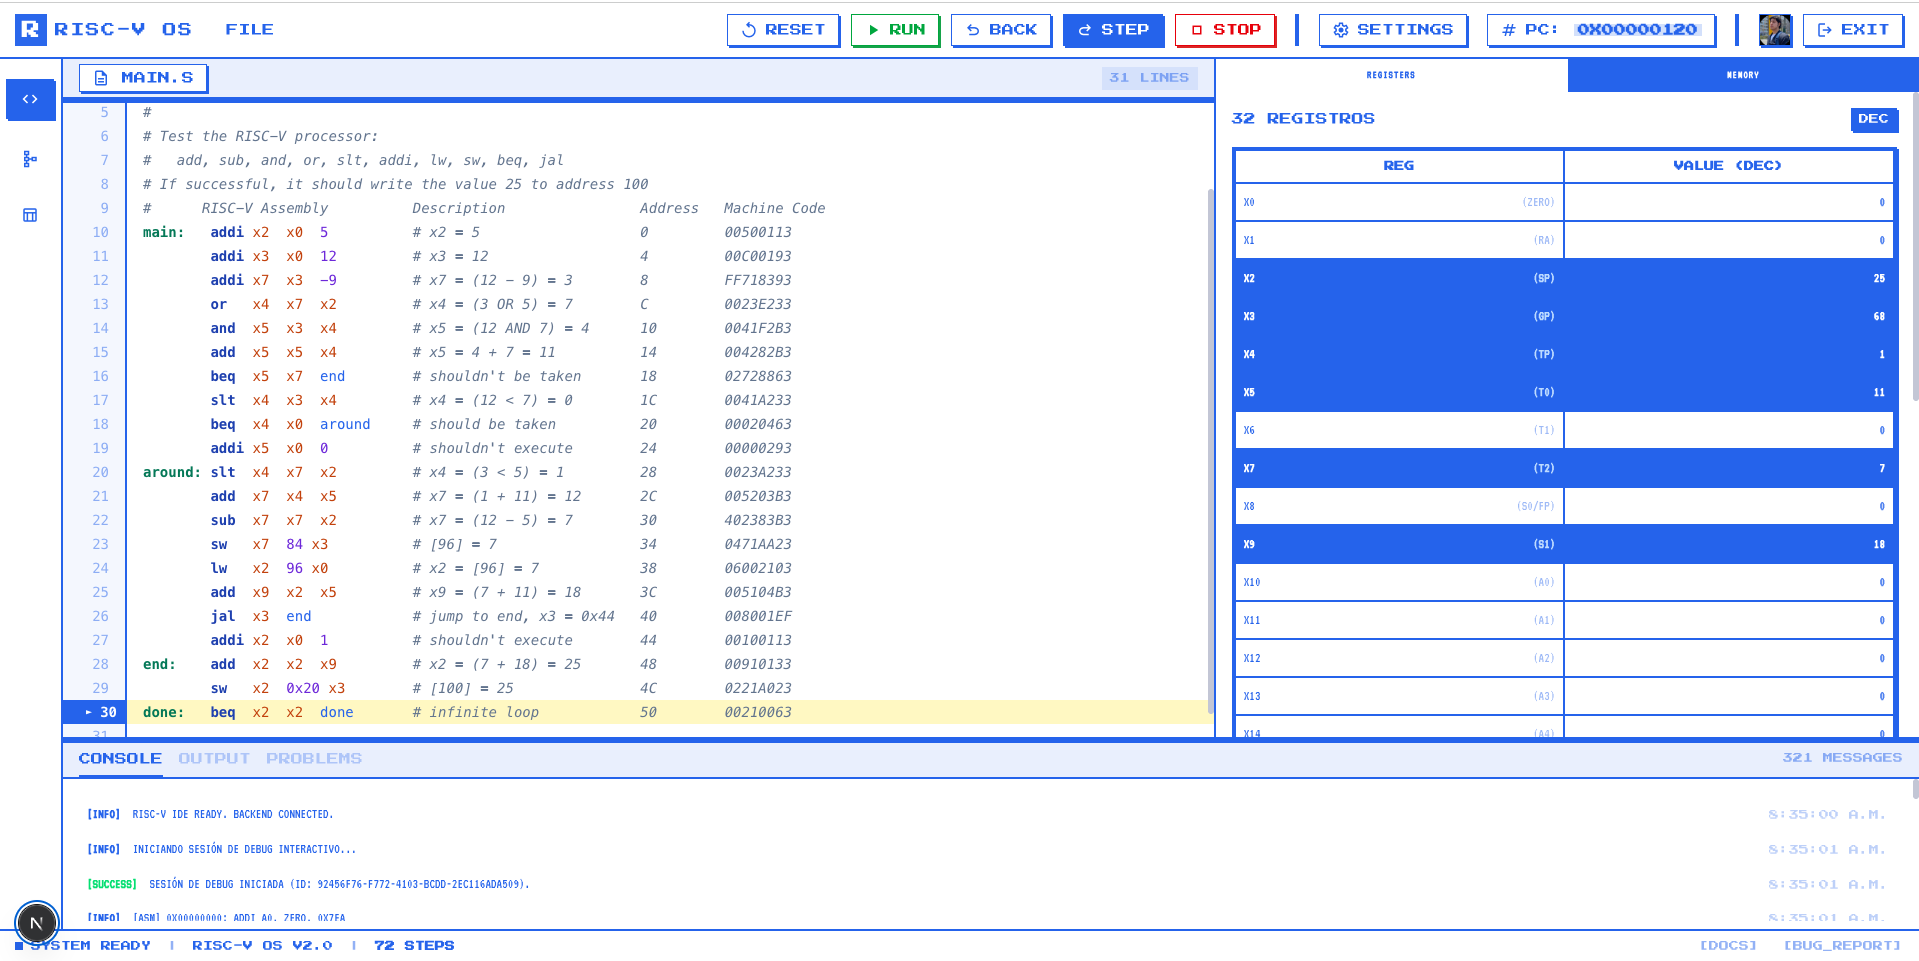
\includegraphics[width=0.95\textwidth]{images/arbol_simetrico.png}
    \caption{Simulación del algoritmo del árbol simétrico recursivo con valor final a0 = 1.}
    \label{fig:arbol_simetrico}
\end{figure}

\subsection{Panel de Datapath y Señales de Control}
El sistema genera el diagrama del datapath y las señales de control correspondientes en tiempo real por cada instrucción ejecutada.

\begin{figure}[H]
    \centering
    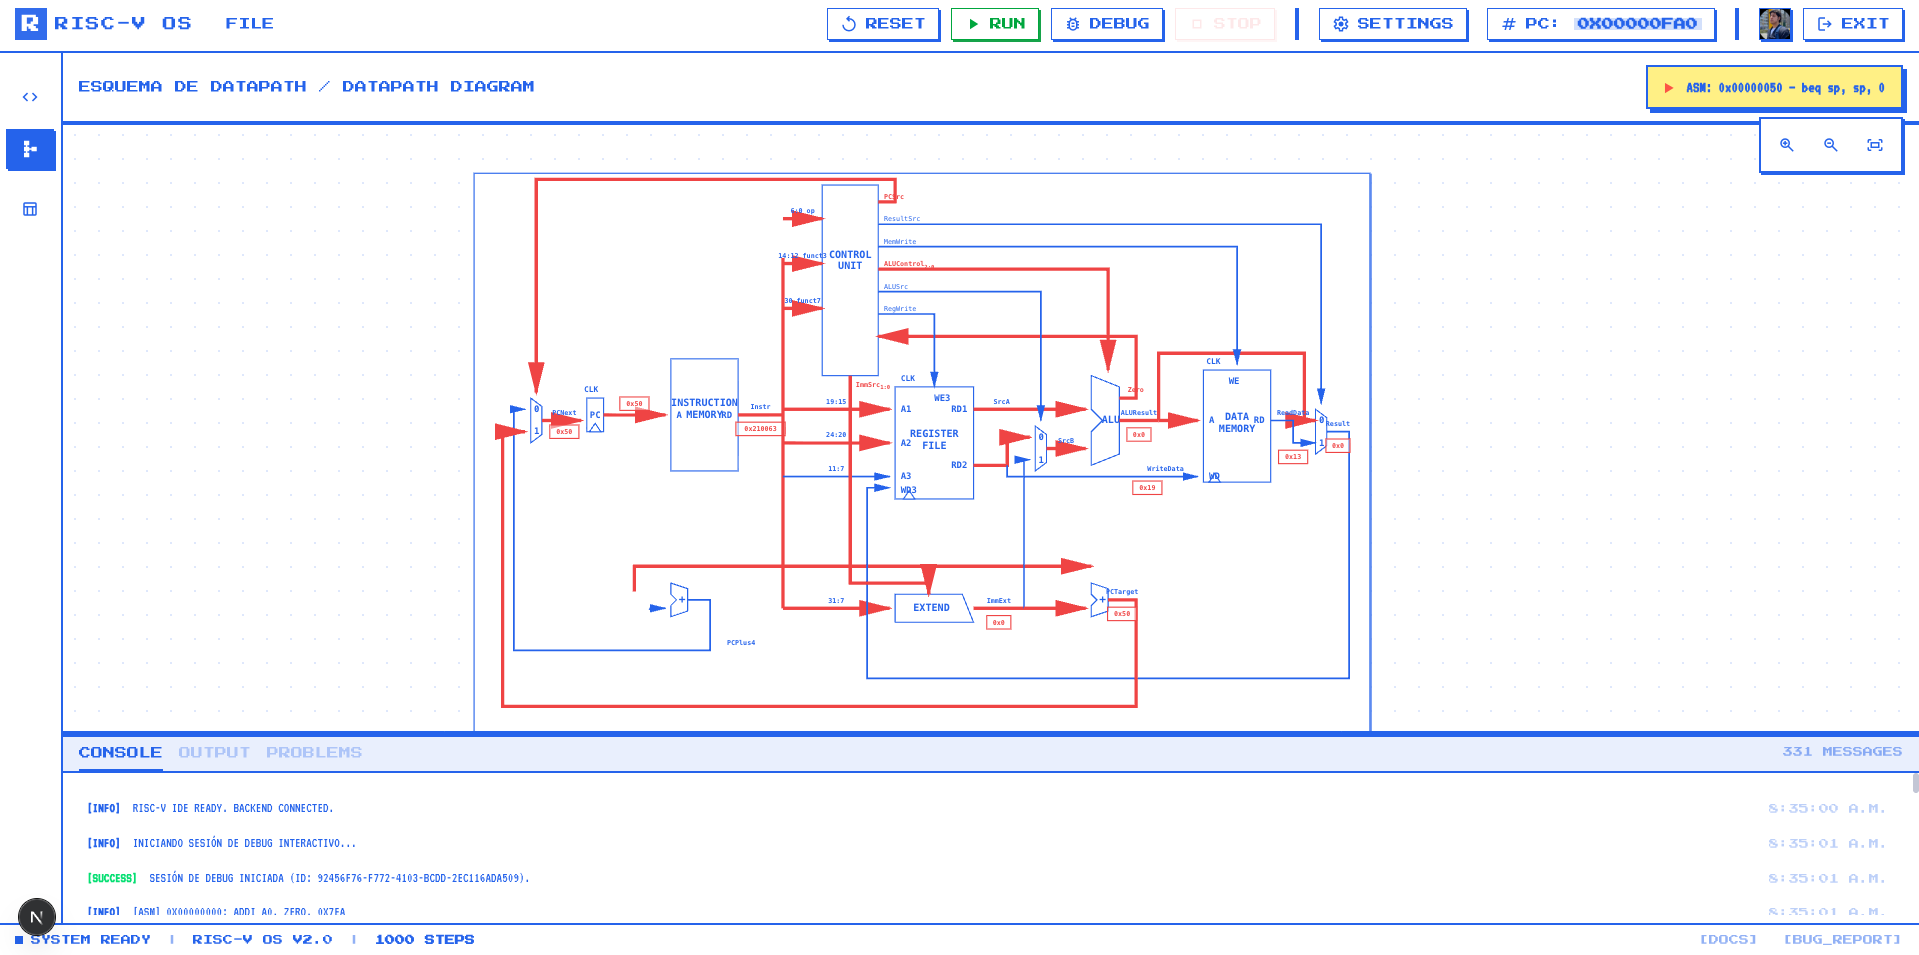
\includegraphics[width=0.95\textwidth]{images/datapath.png}
    \caption{Diagrama esquemático interactivo del Datapath monociclo de la CPU.}
    \label{fig:datapath}
\end{figure}

La unidad de control expone sus señales combinacionales para cada instrucción en una tabla de verdad interactiva.

\begin{figure}[H]
    \centering
    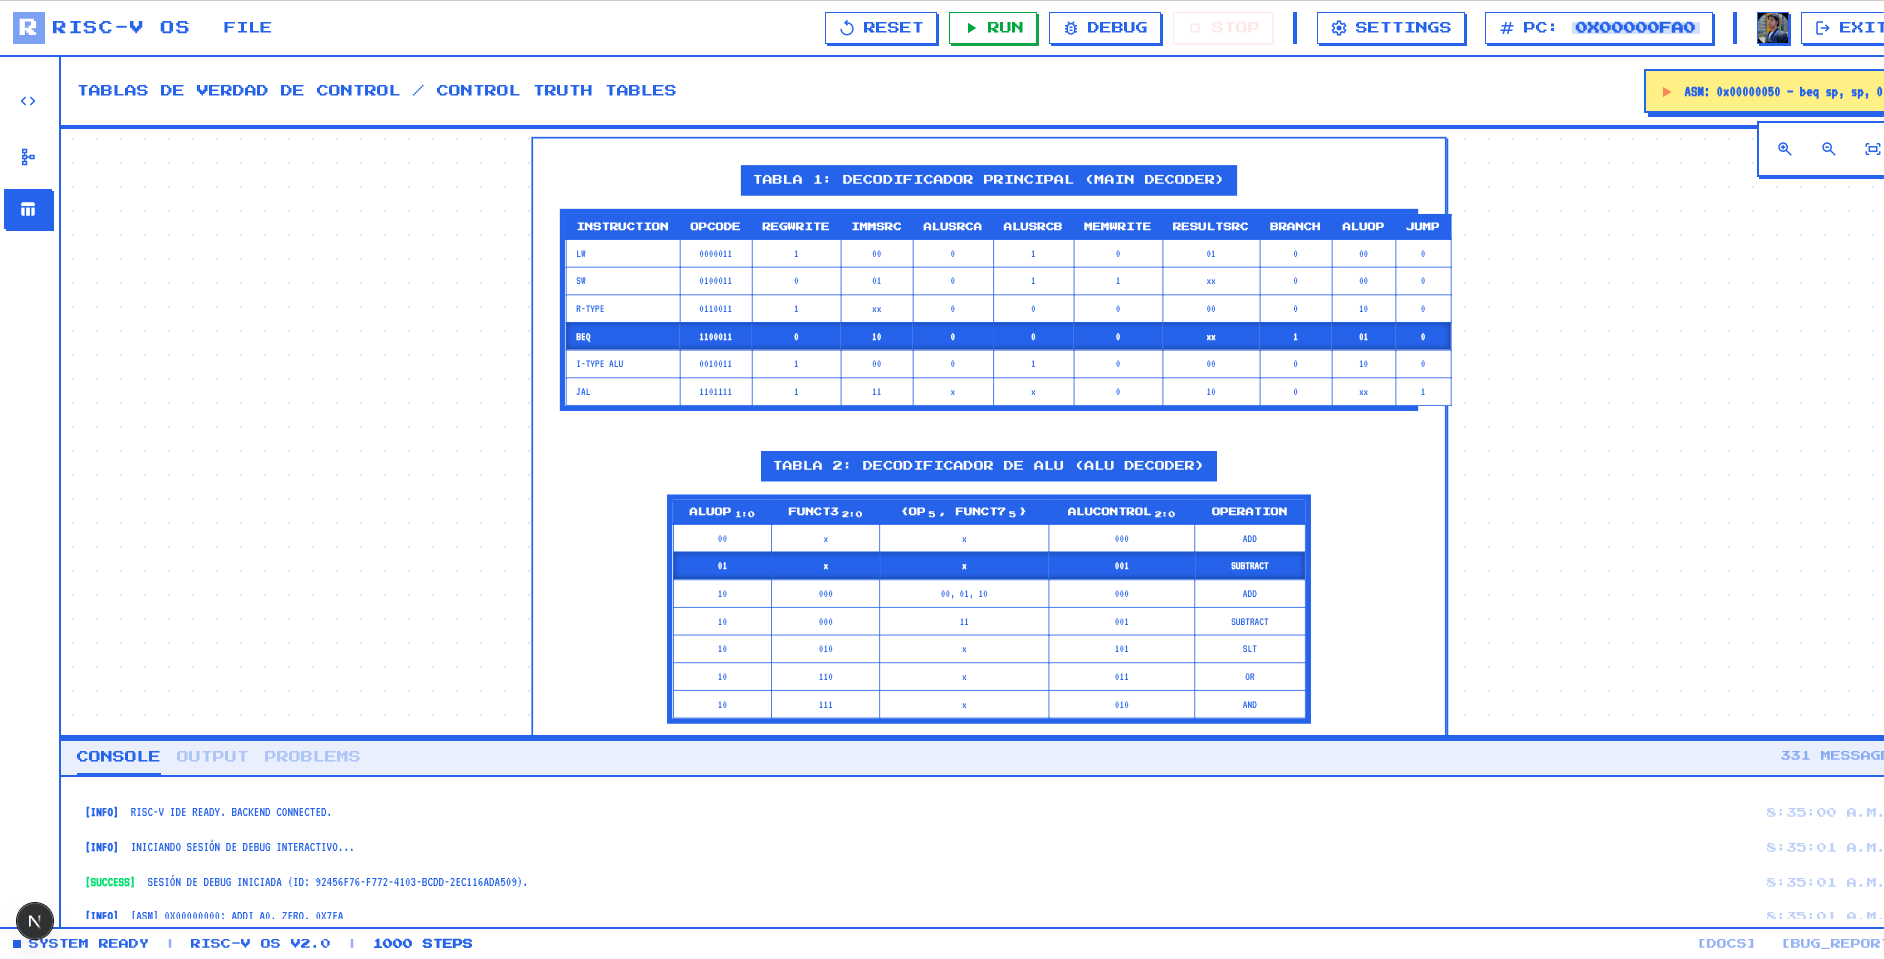
\includegraphics[width=0.95\textwidth]{images/truth_table.png}
    \caption{Tabla de verdad de señales de control del ciclo actual.}
    \label{fig:truth_table}
\end{figure}

---

\section{Trabajo Futuro y Mejoras Propuestas}
Aunque el simulador actual es 100\% funcional y cumple con todos los requerimientos, se proponen las siguientes mejoras de ingeniería para versiones futuras:

\begin{enumerate}
    \item \textbf{Persistencia de Proyectos en Base de Datos:} Implementar el almacenamiento del código fuente y el historial de simulaciones de cada usuario en la base de datos (PostgreSQL) asociada a la cuenta de Google Login del estudiante, permitiendo guardar y cargar proyectos desde la nube.
    \item \textbf{Soporte para Arquitecturas Multi-Cycle y Pipelined:} Expandir la lógica del backend para soportar la ejecución del simulador en modo Multi-Cycle (ejecución por microinstrucciones en múltiples ciclos de reloj) y Pipelined (segmentado con detección de riesgos de datos y control con instrucciones en vuelo).
    \item \textbf{Exportación Detallada a PDF (Reporte de Ejecución):} Añadir un módulo que genere un reporte en PDF de tipo bitácora formal con la explicación paso a paso de las instrucciones ejecutadas, incluyendo volcados del estado del banco de registros y diagramas dinámicos del Datapath para cada ciclo de depuración.
\end{enumerate}

---

\section{Conclusiones}
La traducción de descripciones de hardware en Verilog a implementaciones funcionales en Python demostró ser una excelente estrategia educativa y de ingeniería de software. Permite conservar la fidelidad de la arquitectura física monociclo, facilitando al mismo tiempo la depuración y desarrollo rápido en entornos web interactivos construidos con Next.js y FastAPI. La validación con algoritmos complejos y recursivos de alto consumo de pila (como Quicksort y árboles binarios) consolida la robustez de las unidades aritméticas, lógicas y del manejo little-endian de la memoria implementados.

\end{document}
